\setcounter{deso}{4}
\begin{name}
	{\tenchude}
	{ĐỀ ÔN TẬP CHƯƠNG I}
	{LỚP TOÁN THẦY PHÁT}
	{\thoigian}
\end{name}

\TN
\Opensolutionfile{ans}[ans/ansc1l4-Phan-I]
\begin{ex}%[2-D1B5-SO-17-2425]%[VN-MT-7, VM031]%[2D1N5-1]
 \immini{Đường cong cho trong hình bên là đồ thị của hàm số nào trong các hàm số dưới đây?
 \choice[2]
 {$y=-x^3+2x-1$}
 {$y=-x^3+3x+1$}
 {$y=2x^3-6x+1$}
 {\True $y=x^3-3x+1$}}
 {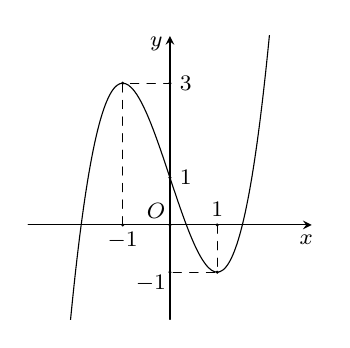
\begin{tikzpicture}[font=\footnotesize,line join=round, line cap=round, >=stealth,scale=0.6] 
 \def \xmin{-3}\def \xmax{3}\def \ymin{-2}\def \ymax{4} 
 \draw[->] (\xmin,0)--(\xmax,0) node[shift=(-110:0.2)] {$x$};
 \draw[->] (0,\ymin)--(0,\ymax) node[shift=(-150:0.2)] {$y$};
 \fill (0,0) circle(1pt) node[shift=(135:0.25)]{$O$}
 (-1,0) circle(1pt) node[shift=(-90:0.2)]{$-1$}
 (1,0) circle(1pt) node[shift=(90:0.2)]{$1$}
 (0,-1) circle(1pt) node[shift=(-150:0.28)]{$-1$}
 (0,1) circle(1pt) node[shift=(0:0.2)]{$1$}
 (0,3) circle(1pt) node[shift=(0:0.2)]{$3$}
 (-1,3) circle(1pt) (1,-1) circle(1pt); 
 \draw[dashed] (-1,0)|-(0,3) (1,0)|-(0,-1);
 \clip (\xmin,\ymin) rectangle (\xmax,\ymax);
 \draw[smooth,samples=100,domain=\xmin:\xmax] plot(\x,{(\x)^3-3*(\x)+1}); 
 \end{tikzpicture}}
 \loigiai{
 Quan sát đồ thị, ta thấy
 \begin{itemize}
 \item Đây là đồ thị của hàm số $y=ax^3+bx^2+cx+d$ $ (a\ne 0)$ có $a > 0$.
 \item Đồ thị hàm số có hai điểm cực trị $(-1;3)$ và $(1;-1)$.
 \end{itemize}
 Vậy đường cong trong hình vẽ là đồ thị hàm số $y=x^3-3x+1$.
 }
\end{ex}

\begin{ex}%[2-D1B5-SO-17-2425]%[VN-MT-7, VM031]%[2D1H5-1]
 \immini{Cho hàm số $y=\dfrac{ax+b}{cx-1}$ có đồ thị như hình vẽ bên dưới. Trong các hệ số $a$, $b$, $c$ có bao nhiêu số dương?
 \choice[2]
 {$0$}
 {\True $2$}
 {$1$}
 {$3$}}
 {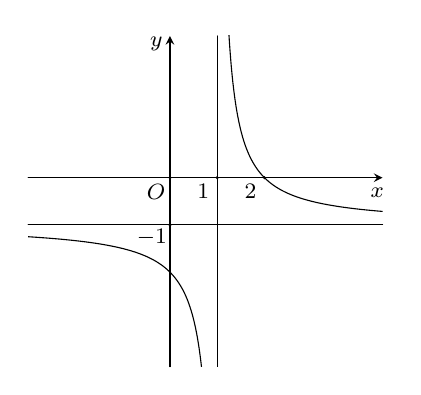
\begin{tikzpicture}[font=\footnotesize,line join=round, line cap=round, >=stealth,scale=0.6] 
 \def \xmin{-3}\def \xmax{4.5}\def \ymin{-4}\def \ymax{3} 
 \draw[->] (\xmin,0)--(\xmax,0) node[shift=(-110:0.2)] {$x$};
 \draw[->] (0,\ymin)--(0,\ymax) node[shift=(-150:0.2)] {$y$};
 \fill (0,0) circle(1pt) node[shift=(-135:0.25)]{$O$}
 (1,0) circle(1pt) node[shift=(-135:0.25)]{$1$}
 (0,-1) circle(1pt) node[shift=(-145:0.28)]{$-1$}
 (2,0) circle(1pt) node[shift=(-135:0.25)]{$2$}; 
 \draw (\xmin,-1)--(\xmax,-1);
 \clip (\xmin,\ymin) rectangle (\xmax,\ymax); 
 \draw[smooth,samples=100,domain=\xmin:0.99] plot(\x,{(-1*(\x)+2)/((\x)-1)});
 \draw[smooth,samples=100,domain=1.01:\xmax] plot(\x,{(-1*(\x)+2)/((\x)-1)}); 
 \draw (1,\ymin)--(1,\ymax);
 \end{tikzpicture}}
 \loigiai{
 \begin{itemize}
 \item Tiệm cận đứng $x=\dfrac{1}{c}=1\Leftrightarrow c=1$.
 \item Tiệm cận ngang $y=\dfrac{a}{c}=-1\Leftrightarrow a=-c\Rightarrow a=-1$.
 \item Đồ thị cắt trục hoành tại $x=2$ nên $2a+b=0$ hay $b=-2a=2$.
 \end{itemize}
 Vậy có hai số dương.
 }
\end{ex}

\begin{ex}%[2-D1B5-SO-17-2425]%[VN-MT-7, VM031]%[2D1H5-1]
 \immini{Đường cong cho trong hình bên là đồ thị của hàm số nào trong các hàm số dưới đây?
 \choice[2]
 {$y=\dfrac{x^2-2x+2}{x+1}$}
 {$y=\dfrac{-x^2+x+2}{x-1}$}
 {\True $y=\dfrac{x^2-x+1}{-x+1}$}
 {$y=\dfrac{-x^2-x+1}{x-1}$}}
 {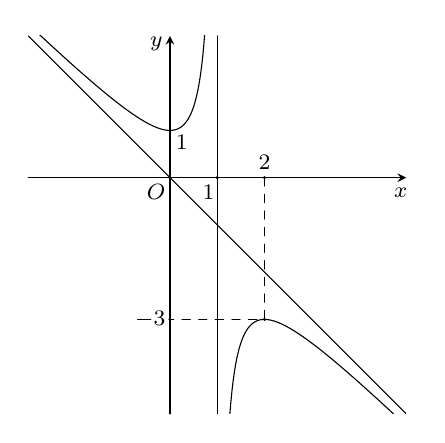
\begin{tikzpicture}[font=\footnotesize,line join=round, line cap=round, >=stealth,scale=0.6] 
 \def \xmin{-3}\def \xmax{5}\def \ymin{-5}\def \ymax{3} 
 \draw[->] (\xmin,0)--(\xmax,0) node[shift=(-110:0.2)] {$x$};
 \draw[->] (0,\ymin)--(0,\ymax) node[shift=(-150:0.2)] {$y$};
 \fill (0,0) circle(1pt) node[shift=(-135:0.25)]{$O$}
 (1,0) circle(1pt) node[shift=(-120:0.22)]{$1$}
 (2,0) circle(1pt) node[shift=(90:0.2)]{$2$}
 (0,1) circle(1pt) node[shift=(-45:0.21)]{$1$}
 (0,-3) circle(1pt) node[shift=(180:0.25)]{$-3$}
 (2,-3) circle(1pt);
 \draw[dashed] (2,0)|-(0,-3);
 \clip (\xmin,\ymin) rectangle (\xmax,\ymax); 
 \clip (\xmin,\ymin) rectangle (\xmax,\ymax);
 \draw[smooth,samples=100,domain=\xmin:0.99] plot(\x,{((\x)^2-1*(\x)+1)/(-1*(\x)+1)}); 
 \draw[smooth,samples=100,domain=1.01:\xmax] plot(\x,{((\x)^2-1*(\x)+1)/(-1*(\x)+1)}); 
 \draw[smooth,samples=100,domain=\xmin:\xmax] plot(\x,{-(\x)}); 
 \draw (1,\ymin)--(1,\ymax);
 \end{tikzpicture}}
 \loigiai{
 \begin{itemize}
 \item Đồ thị hàm số có tiệm cận đứng $x=1$.
 \item Đồ thị hàm số có tiệm cận xiên $y=-x$.
 \item Đồ thị hàm số đi qua điểm $\left(2;-3\right)$.
 \end{itemize}
 Vậy đường cong trong hình vẽ là đồ thị hàm số $y=\dfrac{x^2-x+1}{-x+1}$.
 }
\end{ex}

\begin{ex}%[2-D1B5-SO-17-2425]%[VN-MT-7, VM031]%[2D1H4-1]
 \immini{Cho hàm số $y=\dfrac{ax^2+bx+1}{cx+2}$ có đồ thị như hình vẽ bên dưới. Tính giá trị biểu thức $T=2a+3b-c$.
 \choice[2]
 {$9$}
 {\True $10$}
 {$8$}
 {$11$}}
 {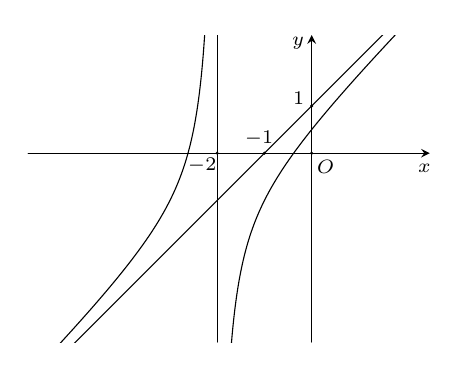
\begin{tikzpicture}[font=\scriptsize, line join=round, line cap=round, >=stealth,scale=0.6] 
 \def \xmin{-6}\def \xmax{2.5}\def \ymin{-4}\def \ymax{2.5} 
 \draw[->] (\xmin,0)--(\xmax,0) node[shift=(-110:0.2)] {$x$};
 \draw[->] (0,\ymin)--(0,\ymax) node[shift=(-150:0.2)] {$y$};
 \fill (0,0) circle(1pt) node[shift=(-45:0.25)]{$O$}
 (-2,0) circle(1pt) node[shift=(-140:0.25)]{$-2$}
 (-1,0) circle(1pt) node[shift=(110:0.2)]{$-1$}
 (0,1) circle(1pt) node[shift=(150:0.19)]{$1$};
 \clip (\xmin,\ymin) rectangle (\xmax,\ymax); 
 \draw[smooth,samples=100,domain=\xmin:-2.01] plot(\x,{((\x)^2+3*(\x)+1)/((\x)+2)}); 
 \draw[smooth,samples=100,domain=-1.99:\xmax] plot(\x,{((\x)^2+3*(\x)+1)/((\x)+2)}); 
 \draw[smooth,samples=100,domain=\xmin:\xmax] plot(\x,{(\x)+1}); 
 \draw(-2,\ymin)--(-2,\ymax);
 \end{tikzpicture}}
 \loigiai{
 \begin{center}
 
 \end{center}
 \begin{itemize}
 \item Đồ thị có tiệm cận đứng $x=-2$. Suy ra $-\dfrac{2}{c}=-2\Leftrightarrow c=1$.
 \item Đồ thị có tiệm cận xiên đi qua hai điểm $(0;1)$ và $(-1;0)$ nên có phương trình \[\dfrac{x}{-1}+\dfrac{y}{1}=1\Leftrightarrow y=x+1.\]
 \end{itemize}
 Khi đó ta có
 \begin{itemize}
 \item $\lim\limits_{x\to+\infty} \dfrac{ax^2+bx+1}{x\left(x+2\right)}=1\Leftrightarrow a=1$;
 \item $\lim\limits_{x\to+\infty} \left(\dfrac{x^2+bx+1}{x+2}-x\right)=\lim\limits_{x\to+\infty}\dfrac{\left(b-2\right)x+1}{x+2}=b-2=1\Leftrightarrow b=3$. 
 \end{itemize}
 Vậy $T=2a+3b-c=2+9-1=10$.
 }
\end{ex}

\begin{ex}%[2-D1B5-SO-17-2425]%[VN-MT-7, VM031]%[2D1N1-2]
 Cho hàm số $f(x)$ có bảng biến thiên như sau
 \begin{center}
 
\begin{tikzpicture}
 \tkzTabInit[nocadre=true,lgt=1.2,espcl=2.5,deltacl=0.5]
 {$x$/0.7,$f'(x)$/0.7,$f(x)$/2}
 {$-\infty$,$0$,$2$,$+\infty$}
 \tkzTabLine{,+,0,-,0,+,}
 \tkzTabVar{-/$-\infty$,+/$1$,-/$-3$,+/$+\infty$}
 \end{tikzpicture}
 \end{center}
 Hàm số đã cho nghịch biến trên khoảng nào dưới đây?
 \choice
 {$(2;+\infty)$}
 {\True $(0;2)$}
 {$(-3;1)$}
 {$(-\infty;1)$}
 \loigiai{
 Dựa vào bảng biến thiên của hàm số, ta có hàm số đã cho nghịch biến trên khoảng $(0;2)$. 
 }
\end{ex}

\begin{ex}%[2-D1B5-SO-17-2425]%[VN-MT-7, VM031]%[2D1H1-1]
 \immini{Hàm số $y=-x^3+3x^2$ đồng biến trên khoảng nào dưới đây?
 \choice
 {$(0;4)$}
 {$(-\infty;0)$}
 {$(2;+\infty)$}
 {\True $(0;2)$} }
 
 \loigiai{
 Ta có $y'=-3x^2+6x=0\Leftrightarrow \hoac{&x=0\\&x=2.}$\\
 Hàm số đồng biến khi $y' > 0$ $\Leftrightarrow 0< x < 2$.
 }
\end{ex}

\begin{ex}%[2-D1B5-SO-17-2425]%[VN-MT-7, VM031]%[2D1N2-2]
 \immini{Cho hàm số $y=f(x)$ xác định và liên tục trên đoạn $[-2; 2]$ và có đồ thị là đường cong trong hình vẽ sau.
 Điểm cực tiểu của đồ thị hàm số $y=f(x)$ là
 \choice[2]
 {$x=1$}
 {$x=-2$}
 {\True $M(1;-2)$}
 {$M(-2;-4)$} }
 {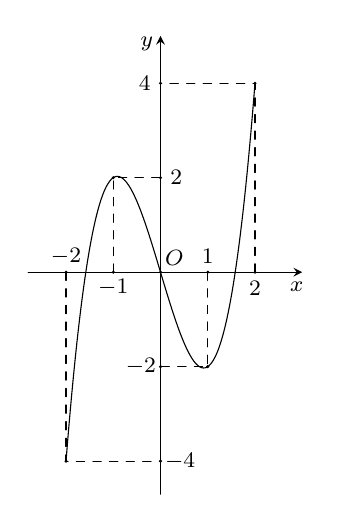
\begin{tikzpicture}[font=\footnotesize,line join=round, line cap=round, >=stealth,scale=0.6] 
 \def \xmin{-2.8}\def \xmax{3}\def \ymin{-4.7}\def \ymax{5} 
 \draw[->] (\xmin,0)--(\xmax,0) node[shift=(-110:0.2)] {$x$};
 \draw[->] (0,\ymin)--(0,\ymax) node[shift=(-150:0.2)] {$y$};
 \fill (0,0) circle(1pt) node[shift=(45:0.25)]{$O$}
 (-2,0) circle(1pt) node[shift=(90:0.2)]{$-2$}
 (-1,0) circle(1pt) node[shift=(-90:0.2)]{$-1$}
 (1,0) circle(1pt) node[shift=(90:0.2)]{$1$}
 (2,0) circle(1pt) node[shift=(-90:0.2)]{$2$}
 (0,-4) circle(1pt) node[shift=(0:0.25)]{$-4$}
 (0,-2) circle(1pt) node[shift=(180:0.25)]{$-2$}
 (0,2) circle(1pt) node[shift=(0:0.2)]{$2$}
 (0,4) circle(1pt) node[shift=(180:0.2)]{$4$}
 (-1,2) circle(1pt) (1,-2) circle(1pt) (-2,-4) circle(1pt) (2,4) circle(1pt);
 \clip (\xmin,\ymin) rectangle (\xmax,\ymax); 
 \draw[smooth,samples=100,domain=-2:2] plot(\x,{4/3*(\x)^3-10/3*(\x)}); 
 \draw[dashed] (-2,0)|-(0,-4) (-1,0)|-(0,2) (1,0)|-(0,-2) (2,0)|-(0,4);
 \end{tikzpicture}}
 \loigiai{
 Dựa vào đồ thị hàm số ta thấy điểm cực tiểu của đồ thị hàm số $y=f(x)$ là $M(1;-2)$.
 }
\end{ex}

\begin{ex}%[2-D1B5-SO-17-2425]%[VN-MT-7, VM031]%[2D1N3-1]
 \immini{Cho hàm số $f(x)$ liên tục trên đoạn $[-2;2]$ có đồ thị như hình vẽ.
 Giá trị nhỏ nhất của hàm số trên đoạn $[-2;2]$ là
 \choice[2]
 {$1$}
 {\True $-1$}
 {$-2$}
 {$3$}}
 {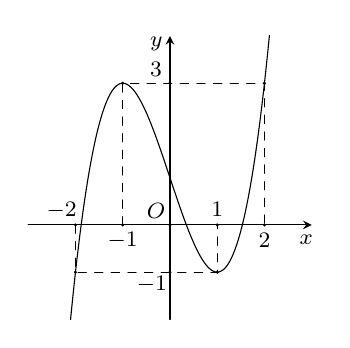
\begin{tikzpicture}[font=\footnotesize,line join=round, line cap=round, >=stealth,scale=0.6] 
 \def \xmin{-3}\def \xmax{3}\def \ymin{-2}\def \ymax{4} 
 \draw[->] (\xmin,0)--(\xmax,0) node[shift=(-110:0.2)] {$x$};
 \draw[->] (0,\ymin)--(0,\ymax) node[shift=(-150:0.2)] {$y$};
 \fill (0,0) circle(1pt) node[shift=(135:0.25)]{$O$}
 (-2,0) circle(1pt) node[shift=(135:0.25)]{$-2$}
 (-1,0) circle(1pt) node[shift=(-90:0.2)]{$-1$}
 (1,0) circle(1pt) node[shift=(90:0.2)]{$1$}
 (2,0) circle(1pt) node[shift=(-90:0.2)]{$2$}
 (0,-1) circle(1pt) node[shift=(-145:0.28)]{$-1$}
 (0,3) circle(1pt) node[shift=(135:0.25)]{$3$}
 (-2,-1) circle(1pt) (1,-1) circle(1pt) (-1,3) circle(1pt) (2,3) circle(1pt);
 \clip (\xmin,\ymin) rectangle (\xmax,\ymax); 
 \draw[smooth,samples=100,domain=\xmin:\xmax] plot(\x,{(\x)^3-3*(\x)+1}); 
 \draw[dashed] (-2,0)--(-2,-1)--(1,-1)--(1,0) (-1,0)--(-1,3)--(2,3)--(2,0);
 \end{tikzpicture}}
 \loigiai{
 Từ đồ thị ta thấy $\min\limits_{[-2;2]} f(x)=f(1)=-1$.
 }
\end{ex}

\begin{ex}%[2-D1B5-SO-17-2425]%[VN-MT-7, VM031]%[2D1H3-1]
 Giá trị nhỏ nhất của hàm số $y=x^2-2x+3$ trên đoạn $[2;4]$ là
 \choice
 {\True $3$}
 {$-1$}
 {$0$}
 {$1$}
 \loigiai{
 \begin{itemize}
 \item $y'=\left(x^2-2x+3\right)'=2x-2$;
 \item $y'=0\Leftrightarrow 2x-2=0\Leftrightarrow x=1\notin [2;4]$.
 \end{itemize}
 Ta có $y(2)=3$; $y(4)=11$.\\
 Vậy $\min\limits_{[2;4]}y=y(2)=3$.
 }
\end{ex}

\begin{ex}%[2-D1B5-SO-17-2425]%[VN-MT-7, VM031]%[2D1N4-1]
 Đồ thị hàm số $y=\dfrac{1+2x}{x-1}$ có đường tiệm cận ngang là
 \choice
 {$x=1$}
 {$y=1$}
 {$x=2$}
 {\True $y=2$}
 \loigiai{
 Ta có $\lim\limits_{x\to \pm \infty} \dfrac{1+2x}{x-1}=\lim\limits_{x\to \pm \infty}\dfrac{\tfrac{1}{x}+2}{1-\tfrac{1}{x}}=2$.\\
 Nên $y=2$ là tiệm cận ngang của đồ thị hàm số.
 }
\end{ex}

\begin{ex}%[2-D1B5-SO-17-2425]%[VN-MT-7, VM031]%[2D1N4-1]
 Đường tiệm cận xiên của đồ thị hàm số $y=\dfrac{x^2-2x+3}{x+1}$ là
 \choice
 {\True $y=x-3$}
 {$y=x+1$}
 {$y=-3x+1$}
 {$x=-3y+1$}
 \loigiai{
 Tập xác định $\mathscr{D}=\mathbb{R}\setminus \{-1\}$.\\
 Phương trình đường tiệm cận xiên có dạng $y=ax+b$.\\
 Trong đó
 \begin{itemize}
 \item $a=\lim\limits_{x\to +\infty} \dfrac{f(x)}{x}=\lim\limits_{x\to +\infty}\dfrac{x^2-2x+3}{x^2+x}=1$;
 \item $b=\lim\limits_{x\to +\infty} \left[f(x)-ax\right]=\lim\limits_{x\to +\infty} \left(\dfrac{x^2-2x+3}{x+1}-x\right)=\lim\limits_{x\to +\infty}\dfrac{-3x+3}{x+1}=-3$.
 \end{itemize}
 Ta cũng có 
 \begin{itemize}
 \item $\lim\limits_{x\to -\infty}\dfrac{f(x)}{x}=1$;
 \item $\lim\limits_{x\to -\infty}\left[f(x)-x\right]=-3$.
 \end{itemize}
 Khi đó $\lim\limits_{x\to \pm\infty} \left[f(x)-(x-3)\right]=\lim\limits_{x\to \pm\infty} \dfrac{6}{x+1}=0$.\\
 Do đó, đồ thị hàm số có tiệm cận xiên là đường thẳng $y=x-3$.
 }
\end{ex}

\begin{ex}%[2-D1B5-SO-17-2425]%[VN-MT-7, VM031]%[2D1H4-1]
 Tổng số đường tiệm cận của đồ thị hàm số $y=\dfrac{\sqrt{x}+1}{3x-9\sqrt{x}+6}$ là
 \choice
 {\True $3$}
 {$4$}
 {$2$}
 {$1$}
 \loigiai{
 Tập xác định $\mathscr{D}=[0;+\infty)\setminus \left\{1;4\right\}$.\\
 Ta có $\lim\limits_{x\to +\infty}\dfrac{\sqrt{x}+1}{3x-9\sqrt{x}+6}=0$.\\
 Nên đồ thị hàm số có $1$ đường tiệm cận ngang là $y=0$.
 \begin{itemize}
 \item $\lim\limits_{x\to 1^+}\dfrac{\sqrt{x}+1}{3x-9\sqrt{x}+6}=\lim\limits_{x\to 1^+} \dfrac{\sqrt{x}+1}{3\left(\sqrt{x}-1\right)\left(\sqrt{x}-2\right)}=+\infty$;
 \item $\lim\limits_{x\to 1^-}\dfrac{\sqrt{x}+1}{3x-9\sqrt{x}+6}=-\infty$.
 \end{itemize}
 Suy ra đường thẳng $x=1$ là $1$ tiệm cận đứng của đồ thị hàm số.
 \begin{itemize}
 \item $\lim\limits_{x\to 4^+} \dfrac{\sqrt{x}+1}{3\left(\sqrt{x}-1\right)\left(\sqrt{x}-2\right)}=+\infty$;
 \item $\lim\limits_{x\to 4^-} \dfrac{\sqrt{x}+1}{3x-9\sqrt{x}+6}=-\infty$.
 \end{itemize}
 Suy ra đường thẳng $x=4$ là $1$ tiệm cận đứng của đồ thị hàm số.\\
 Đồ thị hàm số không có tiệm cận xiên.\\
 Vậy tổng số đường tiệm cận của đồ thị hàm số là $3$.
 }
 \end{ex}
\Closesolutionfile{ans}

\TNTF
\Opensolutionfile{ans}[ans/ansc1l4-Phan-II]
\begin{ex}%[2-D1B5-SO-17-2425]%[VN-MT-7, VM031]%[2D1V5-5]
 \immini{Cho hàm số $y=f(x)$ có đạo hàm trên $\mathbb{R}$ và hàm số $y=f'(x)$ là hàm số bậc ba có đồ thị là đường cong trong hình vẽ.
 \choiceTF
 {Hàm số $y=f(x)$ đồng biến trên khoảng $(-\infty;-2)$}
 {Hàm số $y=f(x)$ có hai điểm cực trị}
 {$f'(2)=4$}
 {\True Hàm số $g(x)=f(x)-\dfrac{1}{2} x^2+x+2024$ đồng biến trên khoảng $\left(-\dfrac{5}{2};-\dfrac{3}{2} \right)$}}
 {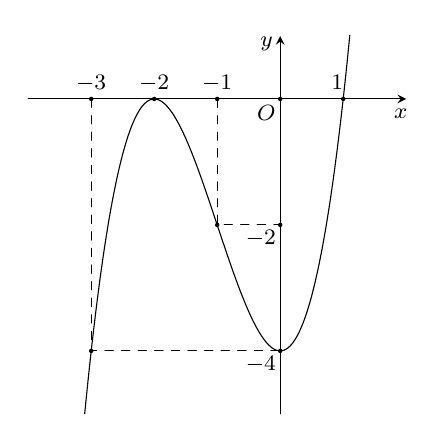
\begin{tikzpicture}[font=\footnotesize,line join=round, line cap=round, >=stealth,scale=0.8] 
 \def \xmin{-4}\def \xmax{2}\def \ymin{-5}\def \ymax{1} 
 \draw[->] (\xmin,0)--(\xmax,0) node[shift=(-110:0.2)] {$x$};
 \draw[->] (0,\ymin)--(0,\ymax) node[shift=(-150:0.2)] {$y$};
 \fill (0,0) circle(1pt) node[shift=(-135:0.25)]{$O$}
 (-3,0) circle(1pt) node[shift=(90:0.2)]{$-3$}
 (-2,0) circle(1pt) node[shift=(90:0.2)]{$-2$}
 (-1,0) circle(1pt) node[shift=(90:0.2)]{$-1$}
 (1,0) circle(1pt) node[shift=(110:0.22)]{$1$}
 (0,-4) circle(1pt) node[shift=(-145:0.3)]{$-4$}
 (0,-2) circle(1pt) node[shift=(-145:0.3)]{$-2$}
 (-1,-2) circle(1pt) (-3,-4) circle(1pt); 
 \clip (\xmin,\ymin) rectangle (\xmax,\ymax); 
 \draw[smooth,samples=100,domain=\xmin:\xmax] plot(\x,{(\x)^3+3*(\x)^2-4}); 
 \draw[dashed] (-3,0)|-(0,-4) (-1,0)|-(0,-2);
 \end{tikzpicture}}
 \loigiai{
 \begin{itemchoice}
 \itemch \textbf{Sai}.\\
 Vì từ đồ thị của hàm số $y=f'(x)$ ta thấy $f'(x)\ge 0$ với $\forall x\ge 1$ nên hàm số đồng biến trên khoảng $(1;+\infty)$.
 \itemch \textbf{Sai}.\\
 Vì từ đồ thị của hàm số $y=f'(x)$ ta thấy $f'(x)$ chỉ đổi dấu một lần qua $x=1$ nên hàm số có một điểm cực trị.
 \itemch \textbf{Sai}.\\
 Từ đồ thị ta có hàm số $f'(x)$ có dạng: $f'(x)=a(x+2)^2 (x-1)$.\\
 Đồ thị hàm số $y=f'(x)$ đi qua $(0;-4)$ nên $-4=a(0+2)^2 (0-1)\Leftrightarrow a=1$.\\
 Vậy $f'(x)=(x+2)^2(x-1)\Rightarrow f'(2)=(2+2)^2 (2-1)=16$.
 \itemch \textbf{Đúng}.\\
 Ta có $g'(x)=f'(x)-x+1=0\Leftrightarrow f'(x)=x-1$.\\
 Vẽ đường thẳng $y=x-1$ trên cùng hệ trục tọa độ với đồ thị hàm số $y=f'(x)$.
 \begin{center}
 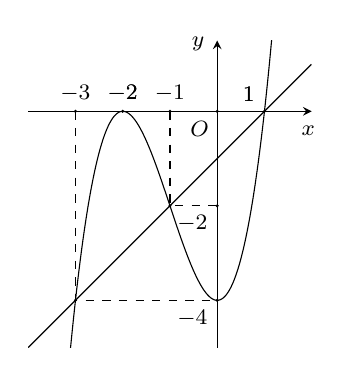
\begin{tikzpicture}[line cap=butt,line join=miter,>=stealth,scale=.6,font=\footnotesize]
 \tikzset{declare function={xmin=-4;xmax=2;ymin=-5;ymax=1.5;
 f(\x)=(\x)^3+3*(\x)^2-4;
 g(\x)=(\x)-1;
 },
 smooth,samples=450
 }
 \draw[->] (xmin,0)--(xmax,0) node[shift={(-100:7pt)}]{$ x $};
 \draw[->] (0,ymin)--(0,ymax) node[shift={(190:7pt)}]{$ y $};
 \fill (0,0) node[shift={(225:9pt)}]{$ O $};
 \draw[dashed](-3,0)node[above]{$-3$}|-(0,-4)node[below left]{$-4$}
 (-1,0)node[above]{$-1$}|-(0,-2)node[below left]{$-2$}
 (-2,0)node[above]{$-2$} (1,0)node[above left]{$1$};
 \fill(-2,0) circle (1pt) node[above]{$-2$} 
 (1,0)circle (1pt) node[above left]{$1$}
 (-3,-4) circle (1pt) (-1,-2) circle (1pt) 
 (1,0) circle (1pt) (0,0) circle (1pt) (0,-4) circle (1pt) (-3,0) circle (1pt) (-1,0) circle (1pt)
 (0,-2) circle (1pt);
 \clip (xmin,ymin) rectangle (xmax,ymax);
 \draw plot[domain=xmin:xmax] (\x, {f(\x)});
 \draw plot[domain=xmin:xmax] (\x, {g(\x)});
 \end{tikzpicture}
 \end{center}
 Khi đó $f'(x)=x-1\Leftrightarrow \hoac{&x=-3\\&x=-1\\&x=1.}$\\
 Bảng biến thiên của hàm số $g(x)$
 \begin{center}
 
\begin{tikzpicture}
 \tkzTabInit[nocadre=true,lgt=1.2,espcl=2.5,deltacl=0.5]
 {$x$/0.7,$f'(x)$/0.7,$f(x)$/2}
 {$-\infty$,$-3$,$-1$,$1$,$+\infty$}
 \tkzTabLine{,-,$0$,+,$0$,-,$0$,+,}
 \tkzTabVar{+/$+\infty$,-/$g(-3)$,+/$g(-1)$,-/$g(1)$,+/$+\infty$}
 \end{tikzpicture}
 \end{center}
 Ta có hàm số $g(x)$ đồng biến trên khoảng $(-3;-1)$ nên $g(x)$ đồng biến trên khoảng $\left(-\dfrac{5}{2};-\dfrac{3}{2} \right)$.
 \end{itemchoice}
 }
\end{ex}

\begin{ex}%[2-D1B5-SO-17-2425]%[VN-MT-7, VM031]%[2D1V2-1]
 Cho hàm số $y=x^3-3x+1$.
 \choiceTF
 {\True Điểm cực tiểu của hàm số là $x=1$}
 {Hàm số đồng biến trên khoảng $(-1;1)$}
 {\True Giả sử hàm số đã cho có hai điểm cực trị là $x_1$; $x_2$. Khi đó giá trị $x_1 \cdot x_2=-1$}
 {Gọi $A$, $B$ lần lượt là điểm cực đại và điểm cực tiểu của đồ thị hàm số. Khi đó, diện tích tam giác $ABC$ là $12$ với $C(-1;2)$}
 \loigiai{
 \begin{itemchoice}
 \itemch \textbf{Đúng}.\\
 Ta có $y'=3x^2-3$\\
 $y'=0\Leftrightarrow 3x^2-3=0\Leftrightarrow \hoac{&x=-1\\&x=1} \Leftrightarrow \hoac{&y(-1)=3\\&y(1)=-1.}$\\
 Ta có bảng biến thiên
 \begin{center}
 
\begin{tikzpicture}
 \tkzTabInit[nocadre=true,lgt=1.2,espcl=2.5,deltacl=0.5]
 {$x$/0.7,$f'(x)$/0.7,$f(x)$/2}
 {$-\infty$,$-1$,$1$,$+\infty$}
 \tkzTabLine{,+,0,-,0,+,}
 \tkzTabVar{-/$-\infty$,+/$3$,-/$-1$,+/$+\infty$}
 \end{tikzpicture}
 \end{center}
 Từ bảng biến thiên ta có điểm cực tiểu của hàm số là $x=1$.
 \itemch \textbf{Sai}.\\
 Vì từ bảng biến thiên ta có hàm số nghịch biến trên khoảng $(-1;1)$.
 \itemch \textbf{Đúng}.\\
 Vì $x_1 \cdot x_2=1\cdot (-1)=-1$.
 \itemch \textbf{Sai}.\\
 Vì $A(-1;3)$, $B(1;-1)$, $C(-1;2)$ nên
 \begin{itemize}
 \item $\left|\overrightarrow{AB}\right|=\sqrt{2^2+(-4)^2}=2\sqrt{5}$;
 \item $\left|\overrightarrow{AC}\right|=\sqrt{0^2+(-1)^2}=1$;
 \item $\cos \widehat{BAC}=\cos\big(\overrightarrow{AB},\overrightarrow{AC}\big)=\dfrac{x_1 x_2+y_1 y_2}{\sqrt{x_1^2+y_1^2} \sqrt{x_2^2+y_2^2}}=\dfrac{2\cdot 0+(-4)(-1)}{\sqrt{2^2+(-4)^2} \sqrt{0^2+(-1)^2}}=\dfrac{2\sqrt{5}}{5}$.
 \item $\sin \widehat{BAC}=\sqrt{1-\cos^2 \widehat{BAC}}=\dfrac{\sqrt{5}}{5}$.
 \item $S_{\triangle ABC}=\dfrac{1}{2}\cdot AB\cdot AC\cdot\sin \widehat{BAC}=\dfrac{1}{2}\cdot 2\sqrt{5}\cdot 1\cdot \dfrac{\sqrt{5}}{5}=1$.
 \end{itemize}
 \end{itemchoice}
 }
\end{ex}

\begin{ex}%[2-D1B5-SO-17-2425]%[VN-MT-7, VM031]%[2D1V3-1]
 Cho hàm số $y=\dfrac{x+m}{x-1}$ ($m$ là tham số thực).
 \choiceTF
 {\True Khi $m=2$ thì giá trị lớn nhất của hàm số trên đoạn $[2;5]$ là $4$}
 {\True Khi $m=2$ thì giá trị nhỏ nhất của hàm số trên đoạn $[2;5]$ là $\dfrac{7}{4}$}
 {Khi $m <-1$ thì giá trị nhỏ nhất của hàm số trên đoạn $[2;4]$ là $y(4)$}
 {Khi $\min\limits_{[2;4]}y=3$ thì giá trị của tham số $m$ là $1\le m < 3$}
 \loigiai{
 Tập xác định $\mathscr{D}=\mathbb{R}\setminus \{1\}$.\\
 Ta có $y'=\dfrac{-1-m}{(x-1)^2}$.
 \begin{itemchoice}
 \itemch \textbf{Đúng}.\\
 Khi $m=2$ thì $y'=\dfrac{-1-2}{\left(x-1\right)^2}=\dfrac{-3}{\left(x-1\right)^2} < 0\; \forall x\in \mathscr{D}\Rightarrow$ hàm số nghịch biến trên từng khoảng xác định, do đó hàm số cũng nghịch biến trên $[2;5]$.\\
 Vậy $\max\limits_{[2;5]}y=y(2)=4$.
 \itemch \textbf{Đúng}.\\
 Khi $m=2$ thì $y'=\dfrac{-1-2}{\left(x-1\right)^2}=\dfrac{-3}{\left(x-1\right)^2} < 0\; \forall x\in \mathscr{D}\Rightarrow$ hàm số nghịch biến trên từng khoảng xác định, do đó hàm số cũng nghịch biến trên $[2;5]$.\\
 Vậy $\min\limits_{[2;5]} y=y(5)=\dfrac{7}{4}$.
 \itemch \textbf{Sai}.\\
 Với $m <-1$ $\Rightarrow-1-m > 0\Rightarrow y' > 0$ nên hàm số đã cho đồng biến trên trên từng khoảng xác định, do đó hàm số cũng đồng biến trên $\left[2;4\right]$ suy ra $\min\limits_{[2;4]}y=y(2)$.
 \itemch \textbf{Sai}.
 \begin{itemize}
 \item Trường hợp 1.\\
 $-1-m > 0\Leftrightarrow m <-1$ $\Rightarrow y' > 0$ nên hàm số đã cho đồng biến trên $[2;4]$.\\
 Khi đó $\min\limits_{[2;4]} y=y(2)\Leftrightarrow 3=2+m\Leftrightarrow m=1\text{ (không thoả mãn)}$.
 \item Trường hợp 2.\\
 $-1-m < 0\Leftrightarrow m >-1$ $\Rightarrow y' < 0$ nên hàm số đã cho nghịch biến trên $[2;4]$.
 \end{itemize}
 Khi đó $\min\limits_{[2;4]} y=y(4)\Leftrightarrow 3=\dfrac{4+m}{3} \Leftrightarrow m=5\text{ (thoả mãn)}$.\\
 Suy ra $m\notin [1;3)$.
 \end{itemchoice}
 }
\end{ex}

\begin{ex}%[2-D1B5-SO-17-2425]%[VN-MT-7, VM031]%[2D1V4-1]
 \immini{Cho hàm số $y=\dfrac{ax+b}{x+c}.(a,b,c\in\mathbb{R})$ có đồ thị như hình vẽ. Khi đó 
 \choiceTF
 {\True Đồ thị hàm số có tiệm cận ngang là $y=-1$}
 {\True Đồ thị hàm số có tiệm cận đứng là $x=1$}
 {$a+b+c=1$}
 {Hàm số đồng biến trên các khoảng xác định}}
 {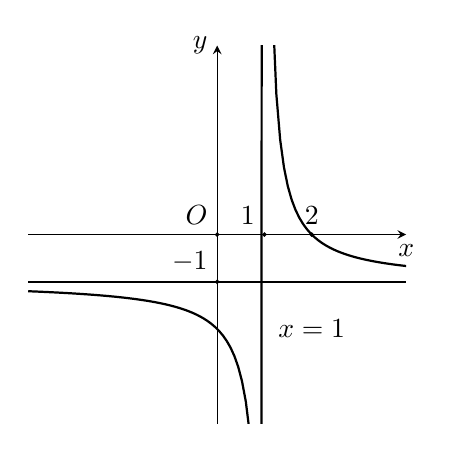
\begin{tikzpicture}[>=stealth,scale=.6]
 \draw[->] (-4,0) --(4,0);
 \draw[->](0,-4)--(0,4);
 \draw (0,0)circle (1pt) node[above left]{$O$};
 \draw (4,0) node[below]{$x$};
 \draw (0,4) node[left]{$y$};
 \draw (1,0)circle (1pt) node[above left]{$1$};
 \draw (0,-1)circle (1pt) node[above left]{$-1$};
 \draw (2,0)circle (1pt) node[above]{$2$};
 \clip (-4,-4) rectangle(4,4);
 \draw[thick,samples=100] plot[domain=-4:4]
 (\x,{(-(\x)+2)/((\x)-1)});
 \draw[thick,samples=100] plot[domain=-4:4]
 (\x,-1);
 \draw (2,-2) node
 {$x=1$};
 \end{tikzpicture}} 
 \loigiai{
 \begin{itemchoice}
 \itemch \textbf{Đúng}.\\
 Dựa vào đồ thị ta thấy đường thẳng $y=-1$ là tiệm cận ngang.
 \itemch \textbf{Đúng}.\\
 Dựa vào đồ thị ta thấy đường thẳng $x=1$ là tiệm cận đứng.
 \itemch \textbf{Đúng}.\\
 Dựa vào đồ thị hàm số ta có 
 \begin{itemize}
 \item Tiệm cận ngang $y=-1\Rightarrow a=-1$.
 \item Tiệm cận đứng $x=1\Rightarrow c=-1$.
 \item Đồ thị hàm số đi qua điểm $(2;0)$ nên $0=\dfrac{-2+b}{2-1}\Rightarrow b=2$. 
 \end{itemize}
 Vậy $a+b+c=-1+2-1=0$.
 \itemch \textbf{Sai}.\\
 Ta có $y=\dfrac{-x+2}{x-1}\Rightarrow y'=\dfrac{-1}{(x-1)^2}< 0$, $\forall x\ne 1$.\\
 Vậy hàm số nghịch biến trên các khoảng xác định.
 \end{itemchoice}
 }
\end{ex}
\Closesolutionfile{ans}

\TNSA
\Opensolutionfile{ans}[ans/ansc1l4-Phan-III]
\begin{ex}%[Đề ôn tập chương1-3]%[Nguyễn Tấn Linh]%[2D1C1-3]
	\immini
	{
	Cho hàm số $y=f(x)$ có đạo hàm liên tục trên $\mathbb{R}$ và có đồ thị $y=f'\left(x\right)$ như hình vẽ. Đặt $g\left(x\right)=f\left(x-m\right)-\dfrac{1}{2}\left(x-m-1\right)^2+2019$, với $m$ là tham số thực. Gọi $S$ là tập hợp các giá trị nguyên dương của $m$ để hàm số $y=g\left(x\right)$ đồng biến trên khoảng $\left(5;6\right)$. Tính tổng tất cả các phần tử trong $S$.\shortans{$14$}
	}
	{
	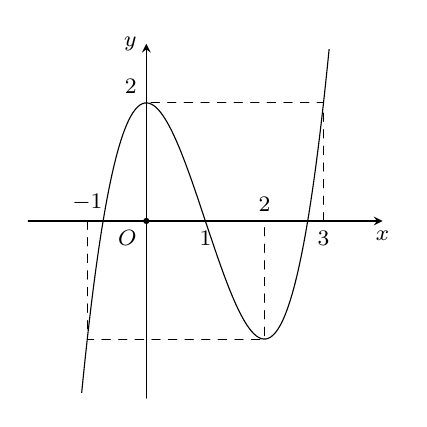
\begin{tikzpicture}[line join = round, line cap = round,>=stealth,font=\footnotesize,scale=.75,declare function={f(\x)=\a*(\x)^3+(\b)*(\x)^2+(\c)*\x+(\d);}]
	\def\xt{-2} \def\xp{4} \def\yd{-3} \def\yt{3}
	\def\a{1}
	\def\b{-3}
	\def\c{0}
	\def\d{2}
	\draw[->] (\xt,0)--(\xp,0) node[below]{$x$};
	\draw[->] (0,\yd)--(0,\yt) node[left]{$y$};
	\fill (0,0) circle (1.5pt) node[below left]{$O$};
	\begin{scope}
	\clip (\xt+0.1,\yd+0.1) rectangle (\xp-0.1,\yt-0.1);
	\draw[samples=150,smooth,domain=\xt:\xp] plot(\x,{f(\x)});
	\end{scope}
	\draw[dashed] (-1,0) node[above]{$-1$}|-(2,-2)--(2,0) node[above]{$2$} (3,0) node[below]{$3$}|-(0,2) node[above left]{$2$};
	\node at (1,0)[below]{$1$};
	\end{tikzpicture}
	}
	\loigiai{
	Xét hàm số $g\left(x\right)=f\left(x-m\right)-\dfrac{1}{2}\left(x-m-1\right)^2+2019$.\\
	$g'\left(x\right)=f'\left(x-m\right)-\left(x-m-1\right)$.\\
	Xét phương trình $g'\left(x\right)=0$.\hfill$\left(1\right)$\\
	Đặt $x-m=t$, phương trình $\left(1\right)$ trở thành $f'\left(t\right)-\left(t-1\right)=0\Leftrightarrow f'\left(t\right)=t-1$.\hfill$\left(2\right)$\\
	Nghiệm của phương trình $\left(2\right)$ là hoành độ giao điểm của hai đồ thị hàm số $y=f'\left(t\right)$ và $y=t-1$.\\
	Ta có đồ thị các hàm số $y=f'\left(t\right)$ và $y=t-1$ như sau
	\begin{center}
	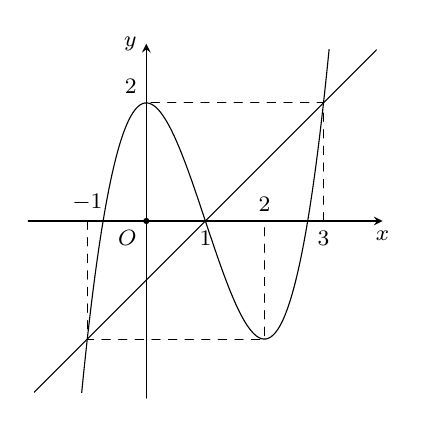
\begin{tikzpicture}[line join = round, line cap = round,>=stealth,font=\footnotesize,scale=.75,declare function={f(\x)=\a*(\x)^3+(\b)*(\x)^2+(\c)*\x+(\d);}]
	\def\xt{-2} \def\xp{4} \def\yd{-3} \def\yt{3}
	\def\a{1}
	\def\b{-3}
	\def\c{0}
	\def\d{2}
	\draw[->] (\xt,0)--(\xp,0) node[below]{$x$};
	\draw[->] (0,\yd)--(0,\yt) node[left]{$y$};
	\fill (0,0) circle (1.5pt) node[below left]{$O$};
	\begin{scope}
	\clip (\xt+0.1,\yd+0.1) rectangle (\xp-0.1,\yt-0.1);
	\draw[samples=150,smooth,domain=\xt:\xp] plot(\x,{f(\x)});
	\draw[samples=150,smooth,domain=\xt:\xp] plot(\x,{\x-1});
	\end{scope}
	\draw[dashed] (-1,0) node[above]{$-1$}|-(2,-2)--(2,0) node[above]{$2$} (3,0) node[below]{$3$}|-(0,2) node[above left]{$2$};
	\node at (1,0)[below]{$1$};
	\end{tikzpicture}
	\end{center}
	Căn cứ đồ thị các hàm số ta có phương trình $\left(2\right)$ có nghiệm là $\hoac{&t=-1 \\&t=1 \\&t=3}\Rightarrow \hoac{&x=m-1 \\&x=m+1 \\&x=m+3.}$\\
	Ta có bảng biến thiên của $y=g\left(x\right)$
	\begin{center}
	
\begin{tikzpicture}
	\tkzTabInit[lgt=2,espcl=2.5]{$x$/1, $y'$/1, $y$/2}{$-\infty$, $m-1$, $m+1$, $m+3$, $+\infty$}
	\tkzTabLine{,-,$0$,+,$0$,-,$0$,+,}
	\tkzTabVar{+/ $+\infty$ , -/ , +/ , -/ , +/ $+\infty$}
	\end{tikzpicture}
	\end{center}
	Để hàm số $y=g\left(x\right)$ đồng biến trên khoảng $\left(5;6\right)$ cần $\hoac{&\heva{&m-1\le 5 \\&m+1\ge 6} \\&m+3\le 5}\Leftrightarrow \hoac{&5\le m\le 6 \\&m\le 2.}$\\
	Vì $m\in \mathbb{N}^*\Rightarrow S=\{1;2;5;6\}\Rightarrow$ Tổng các phần tử trong $S$ bằng $14$.}
	\end{ex}

\begin{ex}%[2-D1B5-SO-17-2425]%[VN-MT-7, VM031]%[2D1V3-6]
 Trong một trò chơi, mỗi đội chơi được phát một tấm bìa hình chữ nhật kích thước 21 cm, 29,5 cm. Nhiệm vụ của mỗi đội là cắt ở bốn góc của tấm bìa này bốn hình vuông bằng nhau, rồi gập tấm bìa lại và dán keo để được một cái hộp không nắp có dạng hình hộp chữ nhật như hình vẽ. 
 \begin{center}
 \begin{tabular}{p{8cm}p{8cm}}
 \begin{tikzpicture}[scale=0.6, font=\footnotesize, line join=round, line cap=round, >=stealth]
 \foreach \x/\y/\pos in {0/0/A, 1/0/B, 1/1/C, 0/1/D, 6/0/A', 0/4/M, 1/4/N, 1/5/P, 0/5/Q, 6/4/M'} \path ($(\x,\y)$) coordinate (\pos); 
 \coordinate (B') at ($(B)+(A')-(A)$);
 \coordinate (C') at ($(C)+(A')-(A)$);
 \coordinate (D') at ($(D)+(A')-(A)$);
 \coordinate (N') at ($(N)+(M')-(M)$);
 \coordinate (P') at ($(P)+(M')-(M)$);
 \coordinate (Q') at ($(Q)+(M')-(M)$);
 \fill[gray!40] (A)--(B)--(C)--(D)--cycle;
 \fill[gray!40] (A')--(B')--(C')--(D')--cycle;
 \fill[gray!40] (M)--(N)--(P)--(Q)--cycle;
 \fill[gray!40] (M')--(N')--(P')--(Q')--cycle;
 \draw (A)--(B')--(P')--(Q)--(A) (D)--(C') (M)--(N') (B)--(P) (A')--(Q');
 \draw[|<->|] ([xshift=-3mm]A)--([xshift=-3mm]Q)node[pos=.5,left]{$21$\,cm};
 \draw[|<->|] ([yshift=3mm]Q)--([yshift=3mm]P')node[pos=.5,above]{$29{,}5$\,cm};
 \end{tikzpicture} & 
 \begin{tikzpicture}[scale=0.6, font=\footnotesize, line join=round, line cap=round, >=stealth]
 \foreach \x/\y/\pos in {0/0/A, -1.8/-1.8/B, 3/-1.8/C} \path ($(\x,\y)$) coordinate (\pos); 
 \coordinate (D) at ($(A)+(C)-(B)$);
 \coordinate (A') at ($(A)+(0,1)$);
 \coordinate (B') at ($(B)+(A')-(A)$);
 \coordinate (C') at ($(C)+(A')-(A)$);
 \coordinate (D') at ($(D)+(A')-(A)$); 
 \draw (A')--(B')--(B)--(C)--(D)--(D')--(A');
 \draw (B')--(C')--(D') (C)--(C');
 \draw [dashed] (B)--(A)--(D) (A)--(A');
 \end{tikzpicture}
 \end{tabular}
 \end{center}
%\begin{center}
% \hspace{3cm}
% 
%\end{center}
 Đội nào thiết kế được chiếc hộp có thể tích lớn nhất sẽ dành chiến thắng. Hãy xác định cạnh của hình vuông bị cắt để thu được hộp có thể tích lớn nhất. (Coi mép dán không đáng kể, kết quả làm tròn đến hàng phần trăm).
 \shortans{4{,}03}
 \loigiai{
 Gọi cạnh của hình vuông bị cắt ở bốn góc là $x$.\\
 Điều kiện $0< 2x < 21\Leftrightarrow 0< x < 10,5$, đơn vị cm.\\
 Ta có kích thước của khối hộp chữ nhật là $x$; $21-2x$;\ $29{,}5-2x$.\\
 Thể tích của khối hộp là $V=(21-2x)\cdot (29{,}5-2x)\cdot x=619{,}5x-101x^2+4x^3=f(x)$.\\
 Thể tích khối hộp lớn nhất khi hàm số $f(x)$ đạt giá trị lớn nhất.\\
 Xét hàm số $f(x)=619{,}5x-101x^2+4x^3$ trên khoảng $(0;10{,}5)$
 \begin{eqnarray*}
 &&f'(x)=12x^2-202x+619{,}5=0\\
 &\Leftrightarrow& \hoac{&x_1 \approx 4{,}03\\&x_2 \approx 12{,}80.}
 \end{eqnarray*}
 Ta có bảng biến thiên
 \begin{center}
 
\begin{tikzpicture}
 \tkzTabInit[nocadre=true,lgt=1.2,espcl=2.5,deltacl=0.5]
 {$x$/0.7,$f'(x)$/0.7,$f(x)$/2}
 {$0$,$x_1$,$10{,}5$}
 \tkzTabLine{,+,0,-,}
 \tkzTabVar{-/$0$,+/$f(x_1)$,-/$f(10{,}5)$}
 \end{tikzpicture}
 \end{center}
 Suy ra $\max\limits_{(0;10{,}5)} f(x)=f(x_1)$.\\
 Vậy cạnh của hình vuông xấp xỉ $4{,}03$ cm.
 }
\end{ex}

\begin{ex}%[2-D1B5-SO-17-2425]%[VN-MT-7, VM031]%[2D1H2-1]
 Điểm cực tiểu $x_{\text{CT}}$ của hàm số $y=x^3+3x^2-9x$ là
 \shortans{1}
 \loigiai{
 Ta có $y'=3x^2+6x-9=0$.\\
 $y'=0 \Leftrightarrow \hoac{&x=1\\&x=-3} \Rightarrow \hoac{&y(1)=-5\\&y(-3)=27.}$\\
 Bảng biến thiên
 \begin{center}
 
\begin{tikzpicture}
 \tkzTabInit[nocadre=true,lgt=1.2,espcl=2.5,deltacl=0.5]
 {$x$/0.7,$f'(x)$/0.7,$f(x)$/2}
 {$-\infty$,$-3$,$1$,$+\infty$}
 \tkzTabLine{,+,0,-,0,+,}
 \tkzTabVar{-/$-\infty$,+/$27$,-/$-5$,+/$+\infty$}
 \end{tikzpicture}
 \end{center}
 Vậy $x=1$ là điểm cực tiểu.
 }
\end{ex}

\begin{ex}%[Vovanle]%[2D1V5-4]
	Một đường thẳng cắt đồ thị hàm số $y=3x^4-4x^2$ tại bốn điểm phân biệt có hoành độ $0;1;a;b$. Tính $S=ab-a-b$. (làm tròn 2 chữ số thậm phân)
	\shortans{$0{,}67$}
	\loigiai{
		Đường thẳng $d$ cắt đồ thị $(C)$ của hàm số $y=f(x)=3x^4-4x^2$ lần lượt tại các điểm $A$, $B$ có hoành độ $0;1$ nên
		$y_A=f(0)=0$; $y_B=f(1)=-1$.\\
		$\Rightarrow A(0;0),\,B(1;-1)$.\\
		Suy ra PTĐT $d$ là $y=-x$.\\
		Phương trình hoành độ giao điểm của $d$ và $(C)$ là
		\allowdisplaybreaks
		\begin{eqnarray*}
			&&3x^4-4x^2=-x\\
			& \Leftrightarrow& 3x^4-4x^2+x=0 \\ 
			& \Leftrightarrow& x\left(3x^3-4x+1\right)=0 \\ 
			& \Leftrightarrow& x(x-1)\left(3x^2+3x-1\right)=0 \\ 
			&\Leftrightarrow& \hoac{& x=0\\& x-1=0 \\& 3x^2+3x-1=0}\Leftrightarrow \hoac{& x=0 \\& x=1\\& x=\dfrac{-3-\sqrt{21}}{6}\\& x=\dfrac{-3+\sqrt{21}}{6}.}
		\end{eqnarray*}
		Từ đó suy ra $a=\dfrac{-3-\sqrt{21}}{6};b=\dfrac{-3+\sqrt{21}}{6}\Rightarrow S=ab-a-b=\dfrac{2}{3}$.\\
		\textbf{Nhận xét:} Do biểu thức $S$ đối xứng nên ta có thể áp dụng định lí Vi-ét để tính nhanh hơn\\
		Cụ thể $a,\,b$ là nghiệm của phương trình $3x^2+3x-1=0$ nên $ab=-\dfrac{1}{3};\,a+b=-1$.\\
		Từ đó suy ra $S=ab-a-b=ab-(a+b)=-\dfrac{1}{3}-(-1)=\dfrac{2}{3}\approx0{,}67$.
	}
\end{ex}

\begin{ex}%[2-D1B5-SO-17-2425]%[VN-MT-7, VM031]%[2D1V3-1]
 Cho hàm số $y=\dfrac{x-m^2-1}{x-m}$ có bao nhiêu giá trị nguyên $m$ thỏa mãn $\max\limits_{[0;4]}y=-6$.
 \shortans{1}
 \loigiai{
 Tập xác định $\mathscr{D}=\mathbb{R}\setminus \{m\}$.\\
 Ta có $y'=\dfrac{m^2-m+1}{\left(x-m\right)^2} > 0$, $\forall x\in \mathscr{D}$ (do $m^2-m+1=\left(m-\dfrac{1}{2} \right)^2+\dfrac{3}{4} > 0$, $\forall m\in \mathbb{R}$).\\
 Do đó hàm số đồng biến trên các khoảng $(-\infty; m)$ và $(m;+\infty)$.\\
 Khi đó $\max\limits_{[0;4]}y=y(4)$.\\
 Để hàm số đã cho có giá trị lớn nhất trên $[0;4]$ bằng $-6$ thì
 \[\heva{&m\notin [0;4]\\&y(4)=-6} \Leftrightarrow \heva{&m\notin [0;4]\\
 &\dfrac{3-m^2}{4-m}=-6} \Leftrightarrow \heva{&m\notin [0;4]\\
 &m^2+6m-27=0} \Leftrightarrow \heva{&m\notin [0;4]\\&\hoac{&m=3\\&m=-9.}} \Leftrightarrow m=-9.
 \]
 Vậy có $1$ giá trị của $m$ thỏa mãn yêu cầu bài toán.
 }
\end{ex}

\begin{ex}%[2-D1B5-SO-17-2425]%[VN-MT-7, VM031]%[2D1V4-2]
 Biết tích các giá trị của tham số $m$ để đồ thị của hàm số $y=\dfrac{2x-4}{x^2+2(m-2)x+m^2+1}$ có đúng $2$ đường tiệm cận là $\dfrac{a}{b}$, $\dfrac{a}{b}$ là phân số tối giản. Tính $P=a^2+b^2$.
 \shortans{85}
 \loigiai{
 Đặt $f(x)=x^2+2(m-2)x+m^2+1$.\\
 Dễ thấy đồ thị không có tiệm cận xiên.\\
 Đồ thị có $1$ tiệm cận ngang là $y=0$ do $\lim\limits_{x\to+\infty} \dfrac{2x-4}{x^2+2(m-2)x+m^2+1}=0$.\\
 Do đó, để đồ thị hàm số có đúng hai đường tiệm cận thì đồ thị hàm số chỉ có đúng $1$ đường tiệm cận đứng.\\
 Khi đó, $f(x)=0$ có $2$ nghiệm phân biệt trong đó có $1$ nghiệm $x=2$ hoặc $f(x)=0$ có nghiệm kép
 \begin{eqnarray*}
 &\Leftrightarrow& \hoac{&\heva{&\Delta' > 0\\&f(2)=0}\\&\Delta '=0} \Leftrightarrow\hoac{&\heva{&(m-2)^2-m^2-1> 0\\&4+2(m-2)\cdot 2+m^2+1=0}\\&(m-2)^2-m^2-1=0}\\
 &\Leftrightarrow&\hoac{&\heva{&-4m+3> 0\\&m^2+4m-3=0} \\&-4m+3=0} \Leftrightarrow \hoac{&\heva{&m < \dfrac{3}{4} \\&m=-2\pm \sqrt{7}} \\&m=\dfrac{3}{4}} \Leftrightarrow \hoac{&m=-2\pm \sqrt{7} \\&m=\dfrac{3}{4}.}
 \end{eqnarray*}
 Vậy tích tất cả các giá trị thực của tham số $m$ là $P=\left(-2+\sqrt{7} \right)\cdot\left(-2-\sqrt{7} \right)\cdot\dfrac{3}{4}=-3\cdot\dfrac{3}{4}=\dfrac{-9}{4}$.\\
 Do đó $a=-9$, $b=4$ nên $P=a^2+b^2=81+4=85$.
 }
\end{ex}
\Closesolutionfile{ans}
% \begin{indapan}
% 	{ans/ansc1l4}
% \end{indapan}

